%!TEX root = ../Thesis.tex
\chapter{Analysis}\label{cha:analysis}
This chapter contains the analysis performed on the case specified in section \ref{sec:cases}. 


    Once the case was defined, one could start looking into the data with more detail. As mentioned, 
    
    
    \section{Anomaly detection}
        \subsection{SVM}
        
        \subsection{KDE}
        
        \subsection{LSTM}
        
    \section{Prepossessing steps}
        \begin{itemize}
            \item Remove data from no operation/ no power production
            \item Remove nan row, must have a complete data matrix 
            \item time differencing to remove trends? mostly for time series forecasting
        \end{itemize}
    \section{Anomaly detection of need raw data signals}
        Show plot and performance comparing the three chosen algorithms. 
    
    \section{Anomaly detection using PCA to reduce feature size}
        Show plot and performance comparing the three chosen algorithms. 
    
    \section{Hourly dataset anlysis?}
        If time and interest this can be added to the thesis 
    

    

    
    not possible to use any timeseries forecasting since the data is not sampled at even frequencies. hense using a regression model and estimating an anomaly based on differences from the sampled and predicted data becomes unvalid. 
    
    bruke kde men det vil antagelig ikkje gje gode resultat sidan samplinga mi er dårlig, og eg ikkje har nok data spredd godt nok utover tilstandsrommet. 

% \section{Unsupervised dimensionallity reduction}\label{sec:dim_reduc}

%     \subsection{PCA}\label{subsec:PCA}


%     \subsection{Kernel PCA}\label{subsec:K_PCA}
    


% \section{Pelton needles}\label{sub:pelton_needles}
%     As mentioned, there was data available from three different power plants with pelton turbines. One of plants had recorded several issues with the needle control, and was used as a case to test early detection of problems with the needle operation. 
    
    
%     \begin{figure}
%         \centering
%         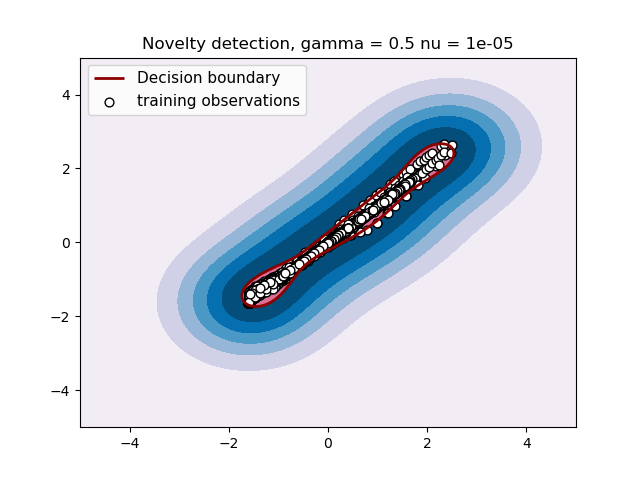
\includegraphics[scale=0.8]{report/figures/analysis/hjartdola/hjar_n2_4_novelty_05_1e-5_train.png}
%         \caption{OCSVM trained on data after overhaul in Mars 2017}
%         \label{fig:my_label}
%     \end{figure}


    
%     \begin{figure}
%         \centering
%         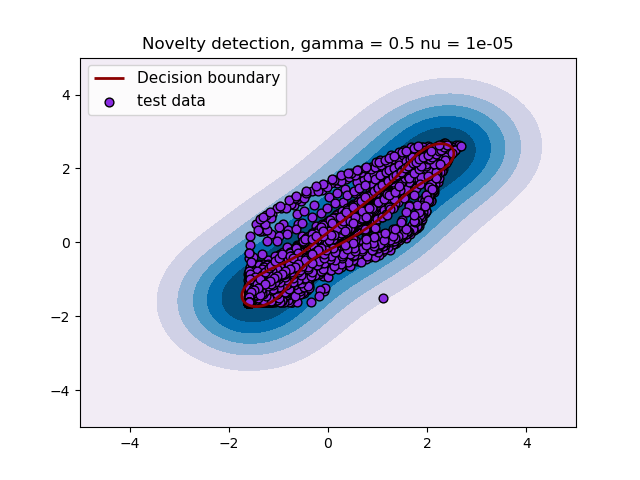
\includegraphics[scale=0.8]{report/figures/analysis/hjartdola/hjar_n2_4_novelty_05_1e-5_test.png}
%         \caption{All process data from before the overhaul}
%         \label{fig:my_label}
%     \end{figure}



